\documentclass[a4paper, 11pt]{article}

%%%%导入包%%%%

\usepackage{xeCJK}
\usepackage{algorithm}
\usepackage{algorithmic}
\usepackage{graphicx}
\usepackage[unicode]{hyperref}
\usepackage{xcolor}
\usepackage{cite}
\usepackage{indentfirst}
\usepackage{amsfonts}
\usepackage{amsmath}
\usepackage{amssymb}
\usepackage{amsthm}
\usepackage{multirow}

%\usepackage{ctex}

\setCJKmonofont{SimHei}  %设置等宽字体
\setCJKsansfont{KaiTi}  %设置楷体
\setCJKmainfont{KaiTi}  %设置缺省中文字体 楷体
\setCJKmonofont{SimHei}  %设置等宽字体
\setmainfont{Arial} % 英文衬线字体
\setmonofont{Arial} % 英文等宽字体
\setsansfont{Arial} % 英文无衬线字体

\setCJKfamilyfont{somefont}{SimHei}
\newcommand*{\somefont}{\CJKfamily{somefont}} 

%%%%%% 设置字号 %%%%%%
\newcommand{\chuhao}{\fontsize{42pt}{\baselineskip}\selectfont}
\newcommand{\xiaochuhao}{\fontsize{36pt}{\baselineskip}\selectfont}
\newcommand{\yihao}{\fontsize{28pt}{\baselineskip}\selectfont}
\newcommand{\erhao}{\fontsize{21pt}{\baselineskip}\selectfont}
\newcommand{\xiaoerhao}{\fontsize{18pt}{\baselineskip}\selectfont}
\newcommand{\sanhao}{\fontsize{15.75pt}{\baselineskip}\selectfont}
\newcommand{\sihao}{\fontsize{14pt}{\baselineskip}\selectfont}
\newcommand{\xiaosihao}{\fontsize{12pt}{\baselineskip}\selectfont}
\newcommand{\wuhao}{\fontsize{10.5pt}{\baselineskip}\selectfont}
\newcommand{\xiaowuhao}{\fontsize{9pt}{\baselineskip}\selectfont}
\newcommand{\liuhao}{\fontsize{7.875pt}{\baselineskip}\selectfont}
\newcommand{\qihao}{\fontsize{5.25pt}{\baselineskip}\selectfont}

%%%% 设置 section 属性 %%%%
\makeatletter
\renewcommand\section{\@startsection{section}{1}{\z@}%
{-1.5ex \@plus -.5ex \@minus -.2ex}%
{.5ex \@plus .1ex}%
{\normalfont\sihao\CJKfamily{hei}}}
\makeatother

%%%% 设置 subsection 属性 %%%%
\makeatletter
\renewcommand\subsection{\@startsection{subsection}{1}{\z@}%
{-1.25ex \@plus -.5ex \@minus -.2ex}%
{.4ex \@plus .1ex}%
{\normalfont\xiaosihao\CJKfamily{hei}}}
\makeatother

%%%% 设置 subsubsection 属性 %%%%
\makeatletter
\renewcommand\subsubsection{\@startsection{subsubsection}{1}{\z@}%
{-1ex \@plus -.5ex \@minus -.2ex}%
{.3ex \@plus .1ex}%
{\normalfont\xiaosihao\CJKfamily{hei}}}
\makeatother

%%%% 段落首行缩进两个字 %%%%
\makeatletter
\let\@afterindentfalse\@afterindenttrue
\@afterindenttrue
\makeatother
\setlength{\parindent}{2em}  %中文缩进两个汉字位

%%%% 下面的命令重定义页面边距,使其符合中文刊物习惯 %%%%
\addtolength{\topmargin}{-54pt}
\setlength{\oddsidemargin}{0.63cm}  % 3.17cm - 1 inch
\setlength{\evensidemargin}{\oddsidemargin}
\setlength{\textwidth}{14.66cm}
\setlength{\textheight}{24.00cm}    % 24.62

%%%% 下面的命令设置行间距与段落间距 %%%%
\linespread{1}
% \setlength{\parskip}{1ex}
\setlength{\parskip}{0.3\baselineskip}

%%%% 正文开始 %%%%
\begin{document}

%%%% 定理类环境的定义 %%%%
\newtheorem{example}{例}             % 整体编号
%\newtheorem{algorithm}{算法}
\newtheorem{theorem}{定理}[section]  % 按 section 编号
\newtheorem{definition}{定义}
\newtheorem{axiom}{公理}
\newtheorem{property}{性质}
\newtheorem{proposition}{命题}
\newtheorem{lemma}{引理}
\newtheorem{corollary}{推论}
\newtheorem{remark}{注解}
\newtheorem{condition}{条件}
\newtheorem{conclusion}{结论}
\newtheorem{assumption}{假设}

%%%% 重定义 %%%%
\renewcommand{\contentsname}{目录}  % 将Contents改为目录
\renewcommand{\abstractname}{摘要}  % 将Abstract改为摘要
\renewcommand{\refname}{参考文献}   % 将References改为参考文献
\renewcommand{\indexname}{索引}
\renewcommand{\figurename}{图}
\renewcommand{\tablename}{表}
\renewcommand{\appendixname}{附录}
%\renewcommand{\algorithm}{算法}

\title{Partial Annotation based CRF}
\author{朱运}

\maketitle

\section{符号定义}

$\mathcal{D}=\{S^j,Y^j\}_{j=1}^N$:表示一个数据集,包含$N$个句子和对应的$N$个人工标注的分词序列。

$S^j=w_1^j...w_i^j...w_{n_j}^j$:表示第$j$个句子,由$n_j$个汉字组成。

$Y^j=y_1^j...y_i^j...y_{n_j}^j$:表示第$j$个句子对应的标签序列。

$\mathcal{T}$:表示标签集合,即隐状态的所有可能取值,$y_i^j \in \mathcal{T}$。

%$\mathcal{V}$:表示字表(vocabulary),即数据$\mathcal{D}$所有汉字的集合,$w_i^j \in \mathcal{V}$。

\section{ 概念定义}

%全标注就是$Y^j$这个标签序列里面每一个位置的tag集合是$\mathcal{T}$子集,且集合里面只有一个tag。
我们以汉语分词任务为例,讲解基于CRF如何实现局部标注,从而得到用于模型更新的loss。
汉语分词任务中,我们采用四标签集\{B, M, E,S\}来表示每个字的分词结果,其中,B、M、E分别代表一个词的开始、中间、结尾,S表示单字成词的字。
那么,$\mathcal{T} = \{B, M, E,S\}$。

全标注是指句子中的每个字都给出了人工标注的分词标签,即 |$Y^j$| = |$S^j$|。
以句子“我是中国人。”为例,我们知道句子的分词答案是“我~~是~~中国人~~。”,那么全标注对应的tag序列是Y =(\{S\},\{S\},\{B\},\{M\},\{E\},\{S\}),如图1所示。 %(\{S\},\{S\},\{B\},\{M\},\{E\},\{S\})
\begin{figure}[htbp]
  \centering
    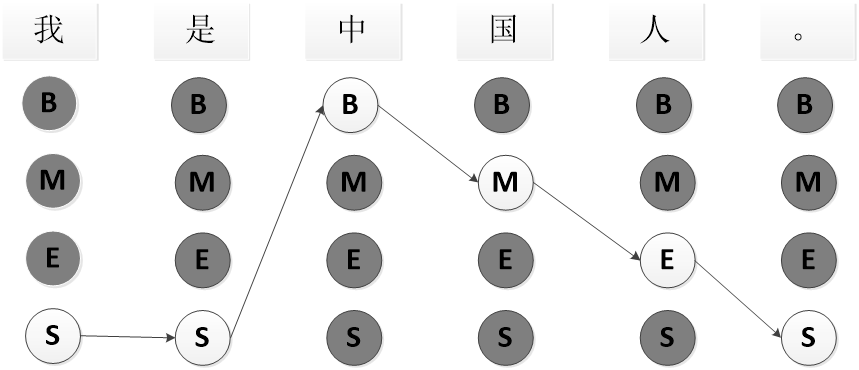
\includegraphics[width=0.8\textwidth]{full_anno_pic.png}
  \caption{“我是中国人”的全标注示例}\label{fig:digit}
\end{figure}

%\newpage

%局部标注就是$Y^j$这个标签序列里面只有给定位置的tag集合是$\mathcal{T}$子集且只有一个tag,其余位置的tag集合是$\mathcal{T}$。
部分标注是指句子中只有部分字的分词标签给出,而其余字的标签没有给出。
我们可以将全标注作为局部标注的一种特殊情形。
假设在句子“我是中国人”中,“中国人”是一个词,其余字的分词信息未知,那么“中国人”对应的tag序列是(B,M,E),
句子中的其他字,我们认为它的标签可能是$\mathcal{T}$中的每个标签,那么句子的标签序列可以表示为(\{B、M、E、S\},\{B、M、E、S\},\{B\},\{M\},\{E\},\{B、M、E、S\}),如图2所示。

\begin{figure}[!htbp]
  \centering
    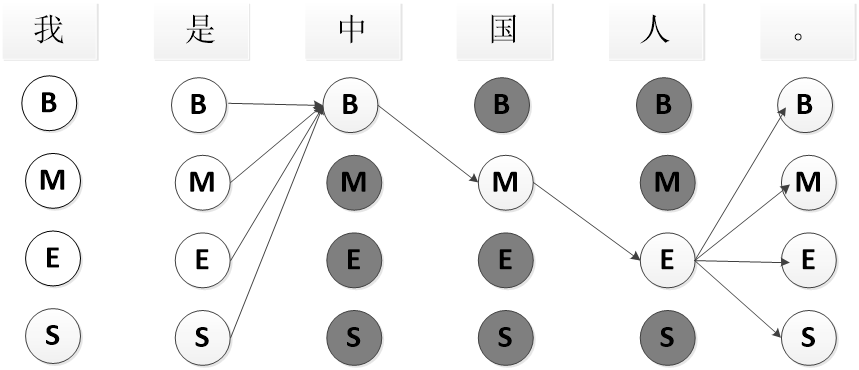
\includegraphics[width=0.8\textwidth]{partial_anno.png}
  \caption{“我是中国人”的局部标注示例,其中,“中国人”是已知的分词信息}\label{fig:digit}
\end{figure}


%模糊标注就是$Y^j$这个标签序列里面只有给定位置的tag集合是$\mathcal{T}$子集且集合里面不只有一个tag,其余位置的tag集合就是$\mathcal{T}$。
模糊标注是指:句子中,每个字或者某些字的标签不是唯一的,即我们允许一个字可以有多个标签。
句子“我是中国人。”,按照不同粒度,“中国人”可以看做一个整体,也可以切分为:“中国”和“人”。
对于句子中的其他字,因为缺少其具体的分词信息,我们认为它的标签可能是$\mathcal{T}$中的每个标签,那么句子的标签序列为(\{B、M、E、S\},~\{B、M、E、S\},~\{B\},~\{M、E\},~\{E、S\},~\{B、M、E、S\}),如图3所示。

\begin{figure}[htbp]
  \centering
    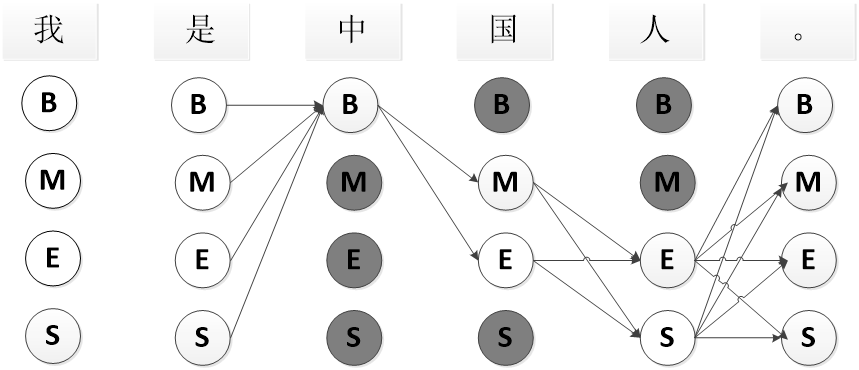
\includegraphics[width=0.8\textwidth]{mohubiaozhu.png}
  \caption{“我是中国人”的模糊标注示例}\label{fig:digit}
\end{figure}

\section{ 公式推导}
我们采用CRF模型来处理分词的序列标注问题。
给定一个输入的字序列,模型的作用是计算序列中每个字赋予每个标签的概率。

全标注中,假设给定的一个句子S = $w_1$...$w_n$,其对应的正确分词序列Y = $y_1$...$y_n$。 
那么,CRF定义句子$S$标注为序列$Y$的概率为:

\begin{equation} \label{eq:CRF_probability}
  \begin{split}
    p(Y|S) = \frac{e^{\textit{Score}(S, Y)}}{Z(S)} \\
  \end{split}
\end{equation}

其中,
\begin{equation} \label{eq:zx}
  \begin{split}
    Z(S) = \sum_{Y' \in \mathcal{T}^n}e^{\textit{Score}(S, Y')} \\
  \end{split}
\end{equation}

%$Y^pL$ = \{(B,B,B,M,E,B),(M,B,B,M,E,B),(E,B,B,M,E,B),(S,B,B,M,E,B),

%\indent\hspace{0.9cm}  (B,M,B,M,E,B),(M,M,B,M,E,B),(E,M,B,M,E,B),(S,M,B,M,E,B),

%\indent\hspace{0.9cm}  (B,E,B,M,E,B),(M,E,B,M,E,B),(E,E,B,M,E,B),(S,E,B,M,E,B),

%\indent\hspace{0.9cm}  (B,S,B,M,E,B),(M,S,B,M,E,B),(E,S,B,M,E,B),(S,S,B,M,E,B)...\}

部分模糊标注,如图3所示,句子中,只有部分词语给定了某个或者某些tag,其余位置标签完全不确定,那么符合图3情况的序列集合:
$Y^p$ = (\{B、M、E、S\},~\{B、M、E、S\},~\{B\},~\{M、E\},~\{E、S\},~\{B、M、E、S\}),
集合$Y^p$里面一共4*4*1*2*2*4 = 256种情况。
其中$Y^p$表示所有可能的序列集合,那么$Y^p$的边缘概率可以表示为

\begin{equation} \label{eq:CRF_partial_probability}
  \begin{split}
  p(Y^p|S) = \sum_{y \in {Y^p} }\frac{e^{\textit{Score}(S, y)}}{Z(S)} \\
  \end{split}
\end{equation}

我们定义${Z^P}$为:
\begin{equation} \label{eq:CRF_partial_Z_probability}
  \begin{split}
    Z_{Y^p} = \sum_{y \in {Y^p} }{e^{{Score}(S, y)}} \\
  \end{split}
\end{equation}

那么局部模糊标注$Y^p$的边缘概率就可以归一化为:
\begin{equation} \label{eq:CRF_normal_partial__probability}
  \begin{split}
    p(Y^p|S) =  \frac{Z_{Y^p}}{Z(S)} \\
  \end{split}
\end{equation}

根据全标注的CRF似然函数
\begin{equation} \label{eq:ll}
  \begin{split}
    LL(\mathcal{D};\mathbf{w}) &= \sum_{j = 1}^N \left [ \textit{Score}(S^j, Y^j) - \mathrm{log}Z(S^j)\right  ]  \\			
  \end{split}
\end{equation}


我们可以得到对应的局部模糊标注的似然函数:
\begin{equation} \label{eq:partial_ll}
  \begin{split}
    LL(\mathcal{D};\mathbf{w}) &= \sum_{j = 1}^N \left [\mathrm{log}Z_{Y^p}(S^j) - \mathrm{log}Z(S^j)\right ] 
  \end{split}
\end{equation}

根据CRF似然函数求解:
\begin{equation} \label{eq:logz-partial}
  \begin{split}
    \frac{\partial{\mathrm{log}Z(S^j)}}{\partial{\mathbf{w}}} &= \sum_{Y' \in \mathcal{T}^n} p(Y'|S)\cdot \mathbf{f}(S^j, Y') 
  \end{split}
\end{equation}

可以得到:
\begin{equation} \label{eq:logZ_Y_L-partial}
  \begin{split}
    \frac{\partial{\mathrm{log}Z_{Y^p}(S^j)}}{\partial{\mathbf{w}}} &= \sum_{Y' \in {Y^p}} p(Y'|S)\cdot \mathbf{f}(S^j, Y') 
  \end{split}
\end{equation}

$Z_{Y^p}$和{Z}的形式以及计算梯度方式很相似,区别在于,在局部模糊标注情况下,我们在计算前向alpha和后向beta的过程中需要加一些约束,将不符合已有标注的情形禁止掉即可。
\begin{equation} \label{eq:alpha_z_y_l}
  \begin{split}
    \alpha^p(k, t) &=\left\{
      \begin{array}{lcl} 
        \sum_{(t) \in {Y^p_k}}e^{\textit{Score}(S, k, t', t)}\cdot \alpha(k - 1, t')	&	&{ t \in {Y^p_k}} \\
      	0		&	& {t \notin {Y^p_k}} 
    \end{array} \right.
  \end{split}
\end{equation}

\begin{equation} \label{eq:beta_z_y_}
  \begin{split}
    \beta^p(k, t) &=\left\{
      \begin{array}{lcl} 
        \sum_{(t,t') \in {Y^p_k}}e^{\textit{Score}(S, k + 1, t, t')}\cdot \beta(k + 1, t')		&	&{t \in {Y^p_k}} \\
      	0		&	& {t \notin {Y^p_k}}  
      \end{array} \right.
  \end{split}
\end{equation}
其中,${Y^p_k}$表示,在局部模糊标注中,第$k$个字对应的所有分词标签。


\section{说明}
全标注,局部标注及模糊标注在训练时,不需要考虑分词标签之间的约束关系(如:B之后只能接E或M,而不能接S),
只有在测试解码时才考虑标签之间的约束关系。










\end{document}































